\section{Experiments}
\label{sec:experiments}
\subsection{Dataset}
We evaluate the proposed method using the Automotive Ethernet traffic from the Controller Area Network and Automotive Ethernet Realistic Data Set (CarDS)~\cite{hellemans2025cards}. CarDS was collected from a commercial electric vehicle manufactured in 2020 and contains time-synchronized traffic from six AE links connecting the gateway electronic control unit (ECU), denoted GWE, to various vehicle components, including the rear-view camera, communication ECUs, and in-vehicle infotainment (IVI) system. In this work, we use the AE traces provided in PCAPNG format, in which attack packets are annotated through packet comments.

The AE traffic was captured using a breakout box installed between the GWE and the AE-connected ECUs. Since CarDS simultaneously records traffic from multiple AE links, a packet propagated through the GWE may be observed more than once. We therefore remove duplicate packet observations caused by GWE propagation from both benign and attack traces before preprocessing and window generation.

For training and validation, we use all 39 benign AE traces provided by CarDS. These traces cover four vehicle operating conditions: standstill, slow driving below 10\,km/h, fast driving above 10\,km/h, and reverse driving. The traces were collected at two restricted sites: a university private parking lot (PPL) and a driving school test area (DSTA). The DSTA emulates public-road conditions through traffic lights, traffic signs, intersections, and roundabouts. Thus, the benign traces capture variations in normal AE traffic across different driving conditions, vehicle states, and recording environments.

We use 31 benign traces for training and the remaining eight for validation. After duplicate removal, preprocessing, and window generation, the training and validation sets contain 5,433,175 and 3,066,673 normal windows, respectively. Sliding windows are constructed independently for each trace, ensuring that no window spans packets from different traces.

CarDS provides 31 Ethernet attack traces, of which 27 are used for performance evaluation. The selected traces comprise five RTP stream replacement traces and 22 Nmap scanning and spoofing traces. The RTP stream replacement attack substitutes frames in the unprotected rear-view camera stream with attacker-controlled video frames. The corresponding traces were recorded under reverse-driving, slow-driving, and standstill conditions.

The Nmap traces target the IVI and emergency communication ECUs and include SYN (\texttt{-sS}), ACK (\texttt{-sA}), and FIN (\texttt{-sF}) scans. The traces cover different port ranges and attacker configurations, including MAC spoofing, IP spoofing, combined MAC and IP spoofing, invalid IP addresses, and VLAN IDs 3 and 4.

Four traces in which attack packets account for no more than $0.01\%$ of all packets are excluded from the performance evaluation: \path{IVI-Nmap_sA_p49000_50000}, \path{IVI-Nmap_sF_p49000_50000}, \path{IVI-Nmap_sS_p1_1024}, and \path{IVI-RestAPI_Crash_vlan3}. These traces contain too few attack samples relative to benign traffic to support a reliable performance evaluation. Table~\ref{tab:dataset} summarizes the experimental dataset constructed from the CarDS AE traces after duplicate removal, preprocessing, and trace-wise sliding-window generation.

\begin{table}[!htbp]
\centering
\caption{Statistics of the experimental dataset constructed from CarDS
AE traces after deduplication and preprocessing.}
\label{tab:dataset}
\footnotesize
\adjustbox{max width=\columnwidth}{%
\begin{tabular}{lrrr}
\toprule
\textbf{Split} & \textbf{Files} & \textbf{Windows} & \textbf{Anomalous} \\
\midrule
Training (normal)           & 31 & 5,433,175 & 0 \\
Validation (normal)         &  8 & 3,066,673 & 0 \\
\midrule
RTP Stream Replacement      &  5 & 1,291,777 &   301,173 \\
Nmap Scanning \& Spoofing   & 22 & 3,811,885 & 1,998,714 \\
\textbf{Total Attack Files} & \textbf{27} & \textbf{5,103,662} & \textbf{2,299,887} \\
\bottomrule
\end{tabular}}
\end{table}

\subsection{Experimental Setup}
\label{sec:experimental_setup}
\noindent\textbf{Implementation Details.}
The proposed model is implemented in PyTorch~\cite{pytorch} and trained for up to 50 epochs with early stopping (patience = 15 epochs) based on validation reconstruction loss. Training is performed on NVIDIA GeForce RTX 3070 and RTX 3080 GPUs. The model is trained exclusively on normal traffic; no labeled attack samples are used at any stage of training. Input representations and the training objective follow the definitions in Section~\ref{sec:methodology}: inputs are preprocessed as specified in Eqs.~\eqref{eq:delta}--\eqref{eq:mask}, and the model is optimized using the asymmetric masked reconstruction loss (Eq.~\ref{eq:loss}) with $\lambda = 5.0$ and $p_{\text{mask}} = 0.20$. The core architecture and training hyperparameters are listed in Table~\ref{tab:hyperparams}.

\noindent\textbf{Evaluation Protocol.}
Each test file is evaluated independently via sliding-window inference with stride 1, and window-level labels follow the any-positive convention: a window is labeled anomalous if at least one of its constituent packets is malicious. We report precision, recall, and F1-score for each attack file. Within each attack category, per-file results are summarized as a macro-averaged subtotal; an overall micro-averaged score is additionally computed by pooling predictions across all 27 attack files. The window-level F1-score serves as the primary metric, with precision and recall reported separately to characterize the precision--recall tradeoff. AUROC and AUPRC are additionally reported as threshold-independent metrics. Anomaly scoring and threshold determination follow the formulations in Section~\ref{sec:scoring} (Eqs.~\ref{eq:score}--\ref{eq:threshold}): a window is flagged as anomalous if its anomaly score $s(\mathbf{X})$ exceeds $\tau$. For a given percentile $p$, $\tau$ is computed solely from the benign validation set; the choice of $p$ itself is made against labeled attacks. In this evaluation $\tau$ is set to the 99th percentile of the validation anomaly score distribution, denoted $P_{99}$; Section~\ref{sec:threshold} motivates that choice and quantifies the cost of selecting $p$ without labels.

\begin{table}[!htbp]
\centering
\caption{Architecture and training hyperparameters used for the proposed method.}
\label{tab:hyperparams}
\footnotesize
\adjustbox{max width=\columnwidth}{%
\begin{tabular}{ll}
\toprule
\textbf{Hyperparameter} & \textbf{Value} \\
\midrule
Window size ($N$)                       & 64 packets \\
Byte length ($L$)                       & 128 bytes \\
Model dimension ($d_{\text{model}}$)    & 128 \\
Transformer layers                      & 3 \\
Attention heads                         & 4 \\
FFN hidden dimension                    & 256 \\
CNN filter progression                  & [128, 128, 128, 64] \\
Positional encoding                     & Time-aware (IPI-based) \\
Dropout rate ($p_{\text{drop}}$)        & 0.1 \\
Mask probability ($p_{\text{mask}}$)    & 0.20 \\
Masked loss weight ($\lambda$)          & 5.0 \\
Optimizer                               & AdamW \\
Learning rate ($\eta$)                  & $1 \times 10^{-4}$ \\
Minimum learning rate                   & $1 \times 10^{-6}$ \\
LR schedule                             & Cosine annealing \\
Weight decay                            & $1 \times 10^{-4}$ \\
Gradient clipping                       & 1.0 \\
Batch size                              & 64 \\
Max epochs ($E$)                        & 50 \\
Early stopping patience                 & 15 epochs \\
\bottomrule
\end{tabular}}
\end{table}

\subsection{Main Results}
\label{sec:main_results}
Table~\ref{tab:main_results} reports the detection performance of the proposed dual-stream masked autoencoder with time-aware positional encoding across all 27 attack files at the $P_{99}$ threshold. The method achieves an overall micro-averaged F1-score of 0.9808 (Precision: 0.9852, Recall: 0.9764; Table~\ref{tab:main_results}), with AUROC of 0.9974 and AUPRC of 0.9972 (Table~\ref{tab:rocprc}). The per-category \emph{Subtotal} rows report the macro-average across files within each category, while the \textbf{Overall} row is micro-averaged across all 27 files; the two aggregation schemes are not directly comparable (see Table~\ref{tab:main_results} caption).

\begin{table*}[!tbp]
\centering
\caption{Detection results of the proposed method (Transformer-CNN with time-aware positional encoding) across 27 attack files (threshold: $P_{99}$), grouped by \textbf{Category} (RTP vs.\ Nmap) and \textbf{Subcategory} (RTP Replace, or, within Nmap, the type of identity spoofing combined with the port scan: MAC, IP, MAC+IP, or none); port range is an experimental parameter and not used for grouping. RD/SD/SS: Reverse/Slow/Standstill driving. \emph{Subtotal} rows report macro-averaged (per-file mean) values within each category; \textbf{Overall} reports micro-averaged (pooled-window) values across all 27 files; the two are not directly comparable.}
\label{tab:main_results}
\footnotesize
\adjustbox{max width=\textwidth}{%
\begin{tabular}{lllccc}
\toprule
\textbf{Category} & \textbf{Subcategory} & \textbf{Attack File} & \textbf{Prec.} & \textbf{Recall} & \textbf{F1} \\
\midrule
\multirow[c]{6}{*}{RTP} & \multirow[c]{5}{*}{RTP Replace}
 & RD-University-RearCamera-ReplaceRTP\_1                    & 0.9270 & 0.9165 & 0.9217 \\
 & & RD-University-RearCamera-ReplaceRTP\_2                    & 0.8459 & 0.8080 & 0.8265 \\
 & & RD-University-RearCamera-ReplaceRTP\_3                    & 0.9317 & 0.8143 & 0.8690 \\
 & & SD-University-RearCamera-ReplaceRTP                       & 0.8531 & 0.8356 & 0.8443 \\
 & & SS-University-RearCamera-ReplaceRTP                       & 0.9349 & 0.8550 & 0.8932 \\
\addlinespace[2pt]
 & & \textit{Subtotal (macro)}                      & \textit{0.8985} & \textit{0.8459} & \textit{0.8709} \\
\midrule
\multirow[c]{26}{*}{Nmap} & \multirow[c]{8}{*}{MAC Spoofing}
 & SS-University-IVI-sA\_MACSpoofing\_vlan3\_1                  & 0.9981 & 0.9983 & 0.9982 \\
 & & SS-University-IVI-sA\_MACSpoofing\_vlan3\_2                  & 0.9996 & 0.9982 & 0.9989 \\
 & & SS-University-IVI-sA\_MACSpoofing\_vlan3\_3                  & 0.9997 & 0.9970 & 0.9984 \\
 & & SS-University-IVI-sS\_MACSpoofing\_vlan3\_1                  & 0.9974 & 0.9989 & 0.9982 \\
 & & SS-University-IVI-sS\_MACSpoofing\_vlan3\_2                  & 0.9994 & 0.9991 & 0.9993 \\
 & & SS-University-IVI-sS\_p49000\_50000\_MACSpoofing\_vlan3\_1   & 0.9623 & 0.9842 & 0.9731 \\
 & & SS-University-IVI-sS\_p49000\_50000\_MACSpoofing\_vlan3\_2   & 0.8864 & 0.9691 & 0.9259 \\
 & & SS-University-IVI-sS\_p49000\_50000\_MACSpoofing\_vlan3\_3   & 0.9419 & 0.9770 & 0.9591 \\
\addlinespace[2pt]
 & & \textit{Subtotal (macro)}                      & \textit{0.9731} & \textit{0.9902} & \textit{0.9814} \\
\cmidrule(l){2-6}
 & \multirow[c]{9}{*}{IP Spoofing}
 & SS-University-IVI-sA\_p49000\_50000\_IPSpoofing\_vlan3          & 0.9818 & 0.9921 & 0.9869 \\
 & & SS-University-Emergency-sS\_IPSpoofing\_vlan4\_1                & 0.9932 & 0.9197 & 0.9550 \\
 & & SS-University-Emergency-sS\_IPSpoofing\_vlan4\_2                & 0.9824 & 0.9519 & 0.9669 \\
 & & SS-University-Emergency-sS\_IPSpoofing\_vlan4\_3                & 0.9899 & 0.9504 & 0.9698 \\
 & & SS-University-Emergency-sS\_IPSpoofing\_vlan4\_4                & 0.9949 & 0.9642 & 0.9793 \\
 & & SS-University-Emergency-sS\_p49000\_50000\_IPSpoofing\_vlan4    & 0.9852 & 0.9138 & 0.9481 \\
 & & SS-University-IVI-sS\_p49000\_50000\_IPSpoofing\_vlan3\_1       & 0.9404 & 0.9816 & 0.9606 \\
 & & SS-University-IVI-sS\_p49000\_50000\_IPSpoofing\_vlan3\_2       & 0.9826 & 0.9920 & 0.9873 \\
 & & SS-University-IVI-sF\_p49000\_50000\_IPSpoofing\_vlan3          & 0.9905 & 0.9872 & 0.9889 \\
\addlinespace[2pt]
 & & \textit{Subtotal (macro)}                      & \textit{0.9823} & \textit{0.9614} & \textit{0.9714} \\
\cmidrule(l){2-6}
 & \multirow[c]{3}{*}{MAC+IP Spoofing}
 & SS-University-Emergency-sS\_p49000\_50000\_MACSpoofing\_IPSpoofing\_vlan4  & 0.9502 & 0.9464 & 0.9483 \\
 & & SS-University-IVI-sS\_MACSpoofing\_IPSpoofing\_InvalidIP\_vlan3            & 0.9998 & 0.9982 & 0.9990 \\
 & & SS-University-IVI-sS\_MACSpoofing\_IPSpoofing\_vlan3                       & 0.9924 & 0.9993 & 0.9958 \\
\addlinespace[2pt]
 & & \textit{Subtotal (macro)}                      & \textit{0.9808} & \textit{0.9813} & \textit{0.9810} \\
\cmidrule(l){2-6}
 & \multirow[c]{2}{*}{No Spoofing}
 & SS-University-Emergency-sS\_p8000\_10000\_vlan4          & 0.9928 & 0.9462 & 0.9689 \\
 & & SS-University-IVI-sS\_p49000\_50000\_vlan3               & 0.9369 & 0.9924 & 0.9639 \\
\addlinespace[2pt]
 & & \textit{Subtotal (macro)}                      & \textit{0.9649} & \textit{0.9693} & \textit{0.9664} \\
\midrule
\multicolumn{3}{l}{\textbf{Overall (micro)}} & \textbf{0.9852} & \textbf{0.9764} & \textbf{0.9808} \\
\bottomrule
\end{tabular}}
\end{table*}

\noindent\textbf{Nmap-based attacks.} The proposed method achieves near-perfect detection on Nmap-based scanning and spoofing attacks, with subcategory-level F1-scores ranging from 0.9664 to 0.9814 (Table~\ref{tab:main_results}). The MAC Spoofing subcategory yields the highest subcategory-level F1 (macro F1 = 0.9814), closely followed by MAC+IP Spoofing (macro F1 = 0.9810); the single best-performing file overall is a SYN-scan MAC spoofing capture (F1 = 0.9993). Detection remains robust even without any spoofing signal: the No Spoofing subcategory, comprising unmodified port scans, still achieves a macro-averaged F1 of 0.9664, the lowest among Nmap-based subcategories but still substantially above the RTP subcategory discussed below.

\noindent\textbf{RTP stream replacement attacks.} Detection of RTP stream replacement attacks remains the most challenging subcategory, with a macro-averaged F1 of 0.8709 (Table~\ref{tab:main_results}). RTP stream replacement preserves the RTP header structure and the inter-packet timing of the original camera stream, differing primarily in payload content. Since both normal and injected RTP streams exhibit high-bandwidth, continuous payload variation with similar inter-arrival patterns, the reconstruction error margin between normal and anomalous traffic is reduced. The proposed method nonetheless achieves per-file F1-scores between 0.8265 and 0.9217 (Table~\ref{tab:main_results}) and a threshold-independent AUPRC of 0.9076 (Table~\ref{tab:rocprc}), indicating that the reconstruction-based anomaly score retains meaningful discriminability even when the attack introduces no temporal anomalies.

Figure~\ref{fig:main_bars} shows the subcategory-level macro-averaged F1-scores from Table~\ref{tab:main_results}, sorted from hardest to easiest. RTP Replace is a clear outlier: its macro F1 (0.8709) falls well below every Nmap subcategory (0.9664--0.9814) and the overall micro-average (0.9808), confirming the categorical asymmetry described above.

\begin{figure}[pos=htbp]
\centering
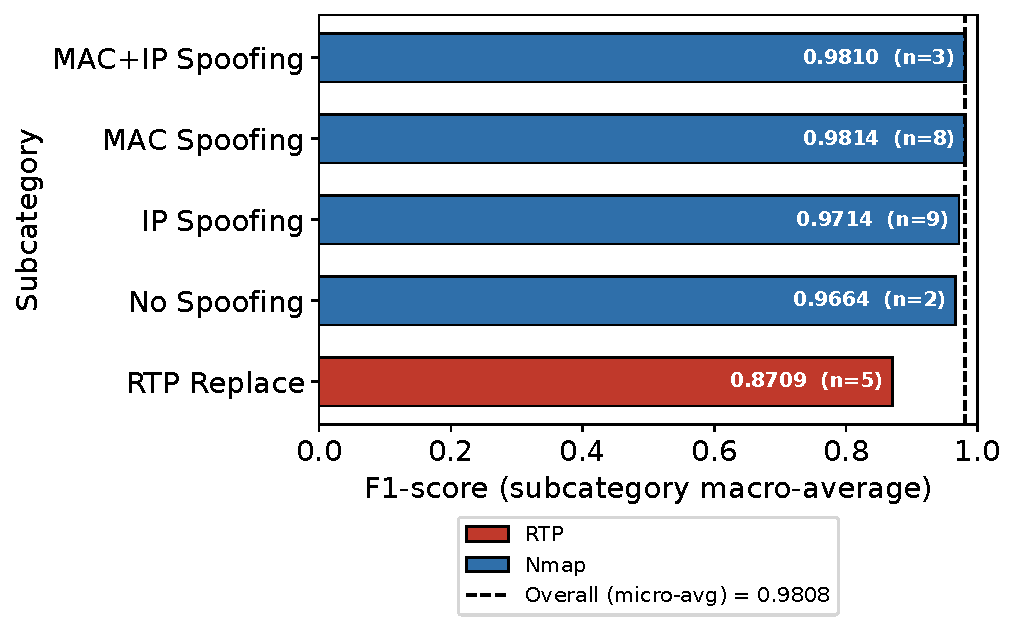
\includegraphics[width=\columnwidth]{figs/main_results_bars.pdf}
\caption{Detection F1 by attack subcategory (macro-average within subcategory) for the proposed method, ordered from hardest to easiest. Bar color indicates the parent category: RTP (red) vs.\ Nmap (blue); $n$ denotes the number of files in each subcategory. The dashed line marks the overall micro-average F1 across all 27 files (0.9808).}
\label{fig:main_bars}
\end{figure}

\noindent\textbf{Threshold-Independent Evaluation.}
To complement the fixed-threshold results above, we additionally report the area under the ROC curve (AUROC) and the area under the precision--recall curve (AUPRC), which characterize detection performance independently of the choice of $\tau$. Figures~\ref{fig:roc_pr}(a) and~\ref{fig:roc_pr}(b) show the ROC and precision--recall curves of the proposed method, aggregated by attack category. Table~\ref{tab:rocprc} summarizes the corresponding AUROC and AUPRC values.

\begin{figure}[pos=htbp]
\centering
\begin{subfigure}[b]{\columnwidth}
    \centering
    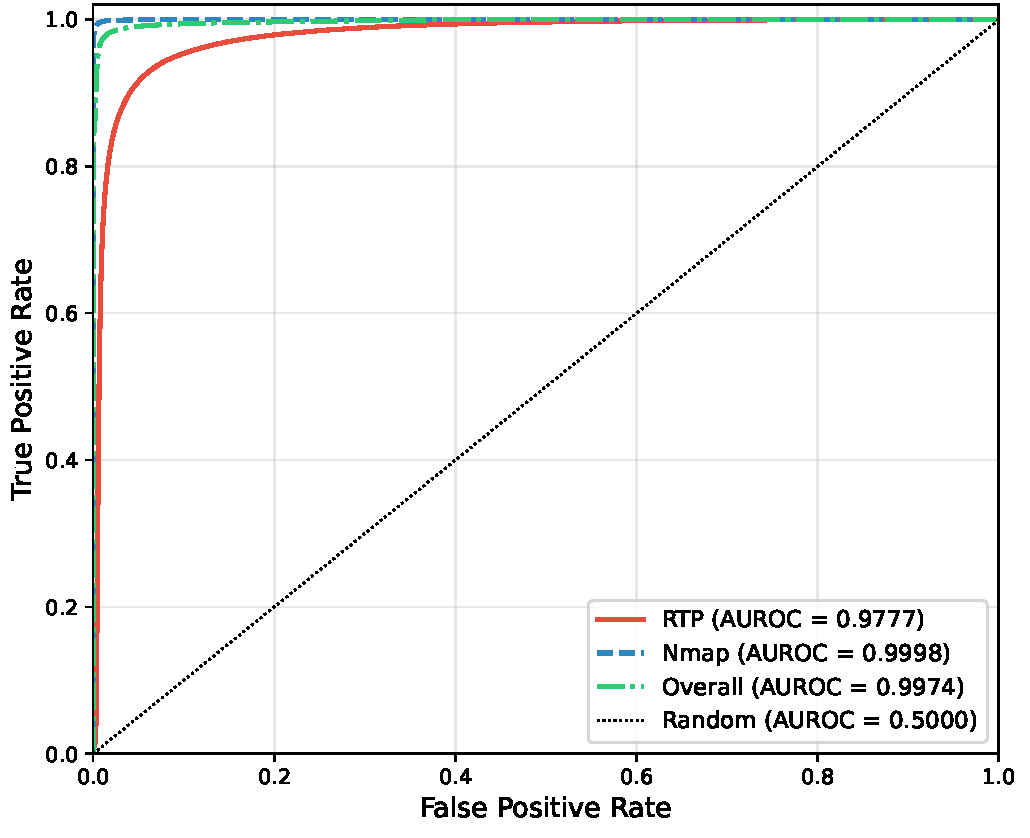
\includegraphics[width=\linewidth]{figs/roc_curve_proposed.pdf}
    \caption{ROC curves}
    \label{fig:roc}
\end{subfigure}

\vspace{2mm}

\begin{subfigure}[b]{\columnwidth}
    \centering
    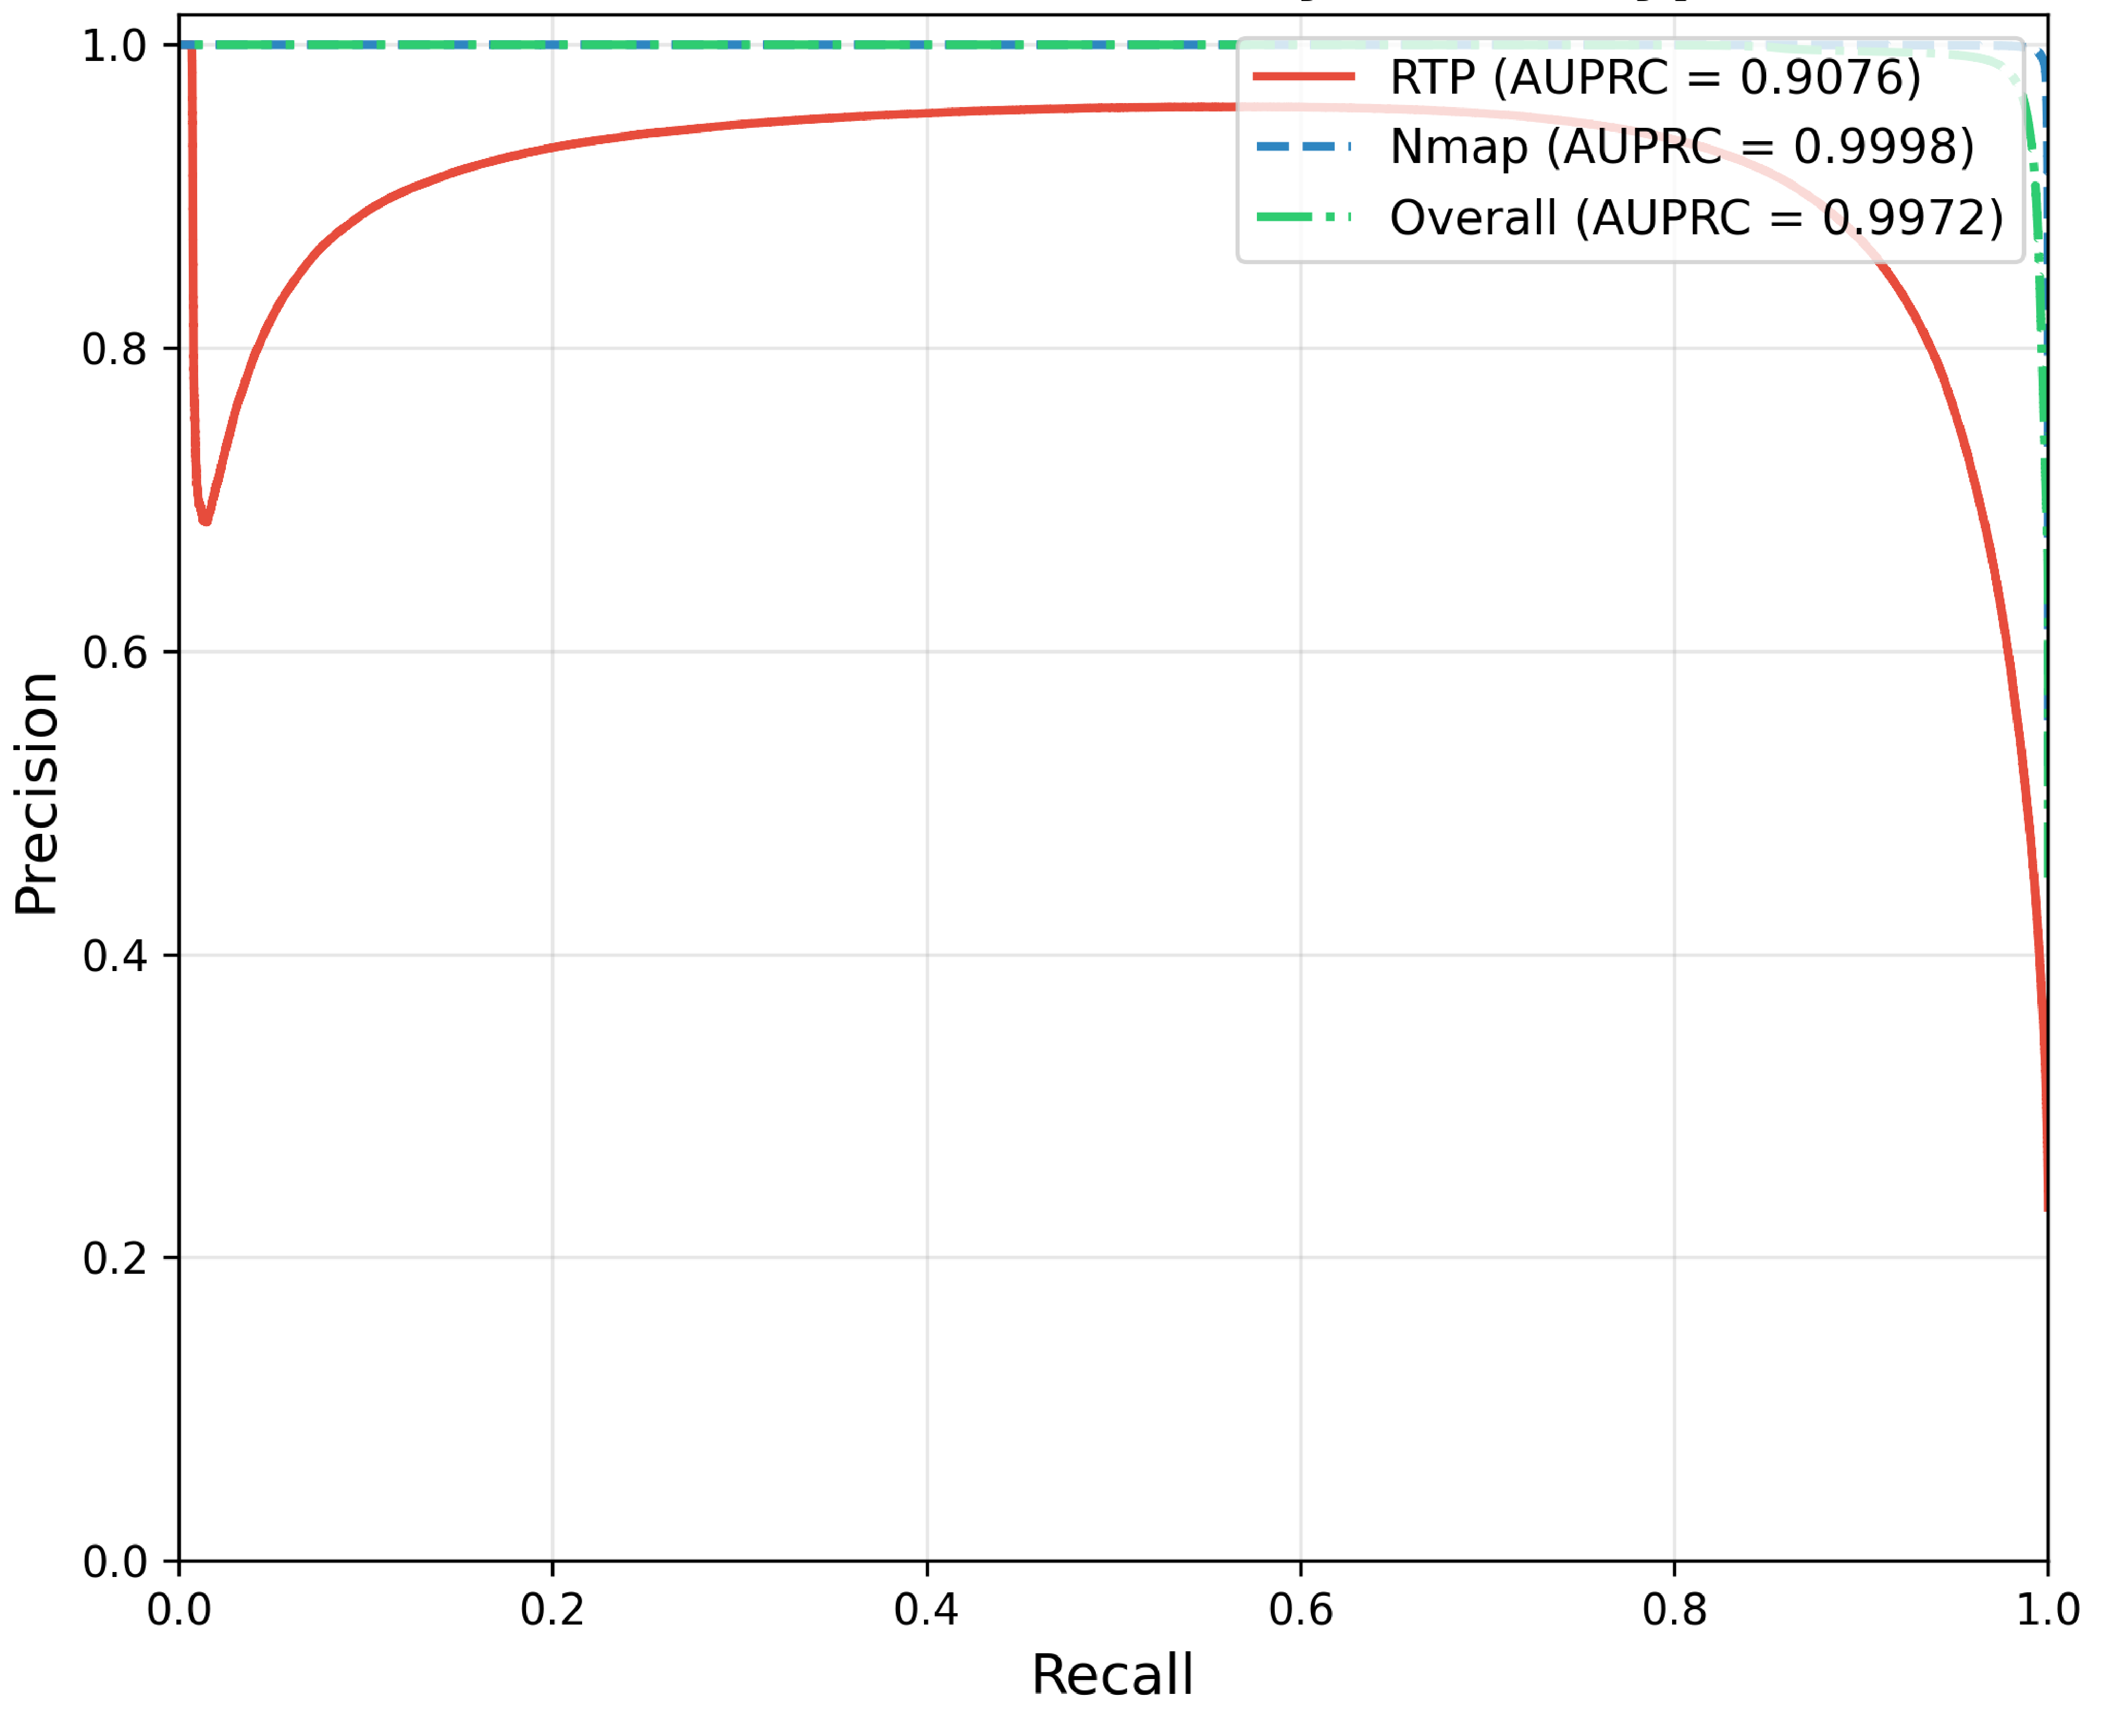
\includegraphics[width=\linewidth]{figs/pr_curve_proposed.pdf}
    \caption{Precision--recall curves}
    \label{fig:pr}
\end{subfigure}
\caption{ROC curves (a) and precision--recall curves (b) for the proposed method (Transformer-CNN with time-aware positional encoding). Each curve is computed by pooling all predictions within the corresponding attack category (micro-average within category).}
\label{fig:roc_pr}
\end{figure}

\begin{table}[!htbp]
\centering
\caption{AUROC and AUPRC for the proposed method (Transformer-CNN with time-aware positional encoding). Category rows: micro-avg within category; \textbf{Overall}: micro-avg across all 27 files.}
\label{tab:rocprc}
\footnotesize
\adjustbox{max width=\columnwidth}{%
\begin{tabular}{lcc}
\toprule
\textbf{Category} & \textbf{AUROC} & \textbf{AUPRC} \\
\midrule
RTP Stream Replacement     & 0.9777 & 0.9076 \\
Nmap Scanning \& Spoofing  & 0.9998 & 0.9998 \\
\midrule
\textbf{Overall (micro)}   & \textbf{0.9974} & \textbf{0.9972} \\
\bottomrule
\end{tabular}}
\end{table}

AUPRC is read against the class prevalence of each split, which is the score a no-skill detector would obtain (Table~\ref{tab:dataset}): 0.524 for the Nmap category, 0.233 for RTP, and 0.451 overall. Consistent with the fixed-threshold results, Nmap-based attacks achieve near-perfect AUROC and AUPRC (0.9998 each; Table~\ref{tab:rocprc}), reflecting a wide margin between normal and anomalous anomaly scores that is robust to the choice of $\tau$. RTP stream replacement attacks attain an AUROC of 0.9777 and an AUPRC of 0.9076 (Table~\ref{tab:rocprc}), indicating stronger separability than the fixed-threshold F1 results alone suggest; the anomaly scores consistently rank attack windows above normal ones, though the F1 gain at any single threshold remains bounded by the intrinsic difficulty of this attack category.

We note a localized dip in the pooled RTP precision--recall curve at low recall (Figure~\ref{fig:roc_pr}(b)), where precision briefly falls from 1.0 to approximately 0.70 before recovering to a plateau above 0.95. This pattern arises from heterogeneity across the five RTP files underlying the pooled curve: per-file AUPRC ranges from 0.8409 (SD-University-RearCamera-ReplaceRTP, the hardest file) to 0.9444 (RD-University-RearCamera-ReplaceRTP\_1, the easiest). The highest-ranked predictions at the most conservative operating points (lowest recall) are dominated by attack windows from the easiest file, for which the error margin from normal traffic is largest. As the threshold is lowered to admit predictions from harder files, a small number of normal windows are interleaved with true positives before recall increases far enough into the harder files' score distributions for precision to recover; this is a pooling artifact of combining five files with unequal detection difficulty into a single curve, rather than evidence of an unstable decision boundary. The subsequent decline at high recall (precision falls to approximately 0.4 as recall approaches 1.0) reflects the conventional PR curve tail effect: achieving recall on the single hardest-to-detect windows in the hardest file requires a threshold permissive enough to also admit a substantial number of normal windows.

\subsection{Comparison with Existing Methods}
\label{sec:baseline}
We compare the proposed method against three representative existing approaches for Automotive Ethernet intrusion detection, each re-implemented and evaluated on the same CarDS traces: (1) a supervised CNN-based detector originally proposed for replay-attack detection in AVTP streams~\cite{jeong2021convolutional}, published in this journal; (2) AERO, an unsupervised real-time anomaly observer for in-vehicle networks that relies on an engineered, protocol-informed feature extractor~\cite{jeong2023aero}; and (3) a feature-aware semi-supervised learning approach for Automotive Ethernet~\cite{shibly2023feature}. Two of these baselines cannot be run without supervision, and we therefore evaluate them under the assumption that labels are available: the CNN detector is given the full attack labels its training procedure requires, and the semi-supervised approach the labeled fraction it assumes. Both are trained and scored under five-fold cross-validation stratified by attack family, so that every family is represented in training while each attack capture is held out exactly once; the reported figures are the resulting out-of-fold predictions, and captures belonging to the same attack scenario are never split across a fold boundary. No supervised baseline is therefore scored on a capture it was trained on. AERO, like the proposed method, is trained on benign traffic only and uses the same benign split. The proposed method receives no attack labels at any stage. This comparison is consequently not label-matched, and the asymmetry runs \emph{against} the proposed method --- most strongly for the fully supervised CNN, and to a lesser degree for the semi-supervised classifier. We report it nonetheless, because the practically relevant question is how far a label-free detector falls short of methods that are granted the supervision they need; the CNN row is therefore best read as a label-privileged reference point rather than as a competing method under equal conditions. Because a supervised classifier, a per-capture-calibrated anomaly detector, and a reconstruction-based scorer do not share a common decision rule, each baseline is additionally evaluated at its own native operating point, and we adopt the threshold-independent AUROC as the primary basis for comparison, reporting F1 for reference only. Table~\ref{tab:baseline} summarizes the learning paradigm, feature representation, and detection performance of each baseline alongside the proposed method.


\begin{table*}[!tbp]
\centering
\caption{Comparison with prior Automotive Ethernet IDS on CarDS. AUROC is the primary, threshold-independent metric; per-row F1 is at each method's native operating point and not directly comparable. Bold marks the proposed method, not the column maximum. $\dagger$Approximate reproduction (no reference implementation); $\ddagger$Best AUROC over the AERO sweep.}
\label{tab:baseline}
\footnotesize
\begin{tabular}{lccccc}
\toprule
\textbf{Method} & \textbf{Paradigm (labels)} & \textbf{Feature} & \textbf{Params} & \textbf{AUROC} & \textbf{F1} \\
\midrule
CNN~\cite{jeong2021convolutional}   & Supervised (100\%)     & Protocol-specific (AVTP) & 1.36M & 0.999           & 0.995 \\
Semi-Sup.~\cite{shibly2023feature}  & Semi-supervised (10\%) & Feature-aware$^\dagger$  & --    & 0.96            & 0.88  \\
AERO~\cite{jeong2023aero}           & Unsupervised (0\%)     & Engineered (multimodal)  & 289k  & 0.81$^\ddagger$ & 0.32  \\
\midrule
Proposed                            & Self-supervised (0\%)  & Raw byte (agnostic)      & 898k  & \textbf{0.9974} & \textbf{0.9808} \\
\bottomrule
\end{tabular}
\end{table*}

\begin{table*}[!tbp]
\centering
\caption{Per-category detection AUROC on CarDS (threshold-independent, micro-avg within category); among the label-free methods, the proposed method alone remains strong on both categories. Bold marks the proposed method, not the column maximum. $\dagger$Approximate reproduction.}
\label{tab:baseline_perattack}
\footnotesize
\begin{tabular}{lcccc}
\toprule
\textbf{Attack category} & \textbf{CNN} & \textbf{Semi-Sup.$^\dagger$} & \textbf{AERO} & \textbf{Proposed} \\
                         & {\footnotesize sup.\ (100\%)} & {\footnotesize semi (10\%)} & {\footnotesize unsup.\ (0\%)} & {\footnotesize self (0\%)} \\
\midrule
RTP Stream Replacement    & 0.999 & 0.74--0.84 & 0.89       & \textbf{0.9777} \\
Nmap Scanning \& Spoofing & 0.997 & $\sim$1.00 & 0.50--0.76 & \textbf{0.9998} \\
\bottomrule
\end{tabular}
\end{table*}

On the threshold-independent AUROC, which is directly comparable across the differing operating points, the proposed method (0.9974) essentially matches the fully supervised CNN detector (0.999) despite using no attack labels, and exceeds both the semi-supervised (0.96) and the unsupervised AERO (0.81) baselines. The comparison with AERO---the only other label-free method, and thus the most directly comparable prior art---is the central result: 0.9974 versus 0.81. We prioritize AUROC over F1 because the three baselines occupy incompatible operating regimes: the supervised CNN emits near-binary sigmoid scores, AERO is calibrated per capture, and both degrade sharply if forced onto the single global percentile threshold used by the proposed reconstruction score. A per-category breakdown (Table~\ref{tab:baseline_perattack}) further reveals that the two prior detectors fail on \emph{complementary} attack categories: AERO collapses to near-random on Emergency/VLAN\,4 Nmap scans (AUROC 0.50), whereas the semi-supervised classifier---strong on scans owing to its partial labels---is weakest on RTP stream replacement (AUROC 0.74--0.84). The proposed method is the only label-free approach that remains strong on both categories (RTP 0.978, Nmap 0.9998).

The proposed method is therefore, to our knowledge, the only approach in this comparison that requires neither labeled attack data nor protocol-specific feature engineering. Section~\ref{sec:baseline_discussion} takes up what that combination buys in a multi-protocol setting.

\subsection{Ablation Study}
\label{sec:ablation}
The ablation study validates four design axes in sequence. We first fix the positional encoding to the conventional sinusoidal scheme ($\mathbf{P}_{\text{enc}} = \mathbf{P}$ in Eq.~\ref{eq:posenc}) and compare stream architectures to identify the optimal backbone, Transformer-CNN (Section~\ref{sec:arch_ablation}). We then fix this backbone and compare the sinusoidal encoding against the proposed time-aware positional encoding (Eq.~\ref{eq:timepe}) to finalize the proposed method (Section~\ref{sec:pe_ablation}). Third, using the finalized proposed method (Transformer-CNN with time-aware PE), we verify that the adopted input byte length (128 bytes) remains optimal (Section~\ref{sec:bytelen_ablation}). Finally, we augment the proposed method with tshark-parsed RTP header fields to probe a protocol-dependent upper bound on detection performance (Section~\ref{sec:rtpheader_ablation}).

\subsubsection{Stream Architecture}
\label{sec:arch_ablation}
Table~\ref{tab:ablation_arch} compares four stream architecture configurations at the $P_{97}$ threshold, all using sinusoidal positional encoding for the content stream. \textbf{Content-only} uses only the Transformer stream on raw byte content without the delta stream. \textbf{CNN-CNN} replaces the Transformer stream with a second residual CNN encoder applied to the content input. \textbf{Transformer-Transformer} replaces the CNN stream with a second Transformer encoder applied to the delta input. \textbf{Transformer-CNN (backbone)} is the dual-stream architecture validated in this section, which is combined with the proposed time-aware positional encoding in Section~\ref{sec:pe_ablation} to form the final proposed method.

\begin{table}[!htbp]
\centering
\caption{Ablation study: stream architecture variants (threshold: $P_{97}$ for all, sinusoidal PE). Overall F1: micro-avg (all 27 files); RTP/Nmap F1: macro-avg within category.}
\label{tab:ablation_arch}
\small
\adjustbox{max width=\columnwidth}{%
\begin{tabular}{lccc}
\toprule
\multirow{2}{*}{\textbf{Variant}} & \multicolumn{3}{c}{\textbf{F1-score}} \\
\cmidrule(l){2-4}
 & Overall & RTP & Nmap \\
\midrule
Content-only                          & 0.9189 & 0.0384 & 0.9222 \\
CNN-CNN                                & 0.9425 & 0.4597 & 0.9474 \\
Trans-Trans                            & 0.9593 & 0.7273 & 0.9560 \\
Trans-CNN (backbone) & \textbf{0.9713} & \textbf{0.7983} & \textbf{0.9570} \\
\bottomrule
\end{tabular}}
\end{table}

The category-level breakdown reveals that architecture choices affect the two attack types differently (Table~\ref{tab:ablation_arch}). The content-only variant achieves an overall F1 of 0.9189 but an RTP F1 of only 0.0384, indicating that without the delta stream the model is essentially unable to detect RTP stream replacement. Its Nmap F1 (0.9222) remains competitive, suggesting that raw byte content alone provides sufficient discriminative signal for scanning and spoofing detection. The dual-stream variants substantially improve RTP detection: CNN-CNN (RTP F1 = 0.4597) and Transformer-Transformer (RTP F1 = 0.7273) both represent large gains over content-only, while Transformer-CNN achieves the highest RTP F1 of 0.7983 among protocol-agnostic configurations. Nmap F1 is similar across all dual-stream variants (0.9474--0.9570), indicating that the architecture choice has limited impact on scanning detection once a delta stream is present.

\subsubsection{Positional Encoding: Sinusoidal vs.\ Time-Aware}
\label{sec:pe_ablation}
Having established Transformer-CNN as the optimal backbone (Section~\ref{sec:arch_ablation}), this section fixes the architecture and varies only the positional encoding scheme. We compare (i) the sinusoidal positional encoding ($\mathbf{P}_{\text{enc}} = \mathbf{P}$ in Eq.~\ref{eq:posenc}) used as the fixed baseline in Section~\ref{sec:arch_ablation} against (ii) the proposed time-aware positional encoding (Eq.~\ref{eq:timepe}). Both variants share the identical Transformer-CNN backbone; the only difference is that the time-aware scheme conditions the content stream's positional signal on the IPI recorded at capture time, rather than on packet rank.

Because the two encoding schemes induce different reconstruction-error distributions on normal traffic, their respective optimal thresholds differ (sinusoidal: $P_{97}$; time-aware: $P_{99}$); we therefore compare both variants at their own empirically selected operating points. Table~\ref{tab:ablation_pe} reports this comparison.

\begin{table}[!htbp]
\centering
\caption{Ablation study: Comparing the conventional sinusoidal positional encoding (baseline) against the proposed time-aware positional encoding, on the fixed Transformer-CNN backbone. Each variant is read at its own best-overall-F1 threshold, selected on the evaluation files, so these are per-variant optima rather than unbiased estimates (Table~\ref{tab:ablation_pe_cat} is threshold-independent). Overall F1: micro-avg (all 27 files); RTP/Nmap F1: macro-avg within category.}
\label{tab:ablation_pe}
\small
\adjustbox{max width=\columnwidth}{%
\begin{tabular}{lcccc}
\toprule
\multirow{2}{*}{\textbf{Variant}} & \multirow{2}{*}{\textbf{Threshold}} & \multicolumn{3}{c}{\textbf{F1-score}} \\
\cmidrule(l){3-5}
 & & Overall & RTP & Nmap \\
\midrule
Sinusoidal (baseline) & $P_{97}$ & 0.9713 & 0.7983 & 0.9570 \\
Time-aware (proposed) & $P_{99}$ & \textbf{0.9808} & \textbf{0.8709} & \textbf{0.9759} \\
\bottomrule
\end{tabular}}
\end{table}

At their respective best operating points, time-aware encoding improves overall F1 from 0.9713 to 0.9808 ($+0.0095$), RTP F1 from 0.7983 to 0.8709 ($+0.0726$), and Nmap F1 from 0.9570 to 0.9759 ($+0.0189$; Table~\ref{tab:ablation_pe}). Because each variant is read at its own empirically selected threshold, these F1 differences are per-variant optima rather than unbiased estimates, and we therefore treat the threshold-independent comparison in Table~\ref{tab:ablation_pe_cat} --- which is unaffected by threshold selection --- as the primary evidence for the encoding change; it shows the same ordering, with RTP AUPRC rising from 0.8675 to 0.9076. The improvement is most pronounced for the RTP category under both views, suggesting that the benefit of time-aware positional conditioning is concentrated on RTP stream replacement detection. From a deployment perspective, a practically important advantage of the time-aware scheme is its threshold robustness: as shown in Section~\ref{sec:threshold}, the sinusoidal model's performance collapses sharply beyond $P_{97}$, whereas the time-aware model remains stable through $P_{99}$, offering a substantially wider usable operating range.

Table~\ref{tab:ablation_pe_cat} further breaks this comparison down by attack category using threshold-independent metrics (AUROC/AUPRC), which are unaffected by the differing threshold scales of the two variants and therefore provide the cleanest evidence of the underlying representational improvement.

\begin{table}[!htbp]
\centering
\caption{AUROC/AUPRC comparison between the conventional sinusoidal positional encoding (baseline) and the proposed time-aware positional encoding (threshold-independent). Category rows: micro-avg within category; Overall: micro-avg across all 27 files.}
\label{tab:ablation_pe_cat}
\small
\adjustbox{max width=\columnwidth}{%
\begin{tabular}{lcccc}
\toprule
\multirow{2}{*}{\textbf{Category}} & \multicolumn{2}{c}{\textbf{Sinusoidal (baseline)}} & \multicolumn{2}{c}{\textbf{Time-aware (proposed)}} \\
\cmidrule(lr){2-3}\cmidrule(l){4-5}
 & AUROC & AUPRC & AUROC & AUPRC \\
\midrule
RTP             & 0.9721 & 0.8675 & \textbf{0.9777} & \textbf{0.9076} \\
Nmap            & 0.9998 & 0.9998 & 0.9998 & 0.9998 \\
\midrule
\textbf{Overall (micro)} & 0.9973 & 0.9968 & \textbf{0.9974} & \textbf{0.9972} \\
\bottomrule
\end{tabular}}
\end{table}

Nmap detection is already near-saturated under sinusoidal encoding (AUROC/AUPRC $\approx 0.9998$) and remains unchanged with time-aware encoding, indicating that byte-level scanning and spoofing signatures are already well captured by the content and delta streams without timing information. RTP stream replacement, in contrast, shows a clear improvement in threshold-independent metrics: AUPRC increases from 0.8675 to 0.9076 ($+0.0401$), a substantially larger gain than the corresponding AUROC improvement ($+0.0056$), consistent with AUPRC's greater sensitivity to precision--recall tradeoffs under class imbalance. This gain is notable because RTP stream replacement does not itself perturb inter-packet timing (Section~\ref{sec:main_results}), yet the introduction of IPI-based positional conditioning improves separability. Possible mechanisms are discussed in Section~\ref{sec:discussion}.

\subsubsection{Input Byte Length}
\label{sec:bytelen_ablation}
Using the finalized proposed method (Transformer-CNN with time-aware positional encoding, Section~\ref{sec:pe_ablation}), we verify that the adopted 128-byte input length remains optimal. Table~\ref{tab:ablation_bytes} compares three input byte length configurations: 64, 128, and 256 bytes per packet.

\begin{table}[!htbp]
\centering
\caption{Ablation study: input byte length, evaluated on the proposed method (Transformer-CNN, time-aware PE). Each variant is read at its own best-overall-F1 threshold, selected on the evaluation files, so these are per-variant optima rather than unbiased estimates (Table~\ref{tab:ablation_pe_cat} is threshold-independent). Overall F1: micro-avg (all 27 files); RTP/Nmap F1: macro-avg within category.}
\label{tab:ablation_bytes}
\small
\adjustbox{max width=\columnwidth}{%
\begin{tabular}{lcccc}
\toprule
\multirow{2}{*}{\textbf{Byte Length ($L$)}} & \multirow{2}{*}{\textbf{Threshold}} & \multicolumn{3}{c}{\textbf{F1-score}} \\
\cmidrule(l){3-5}
 & & Overall & RTP & Nmap \\
\midrule
64 bytes             & $P_{99.9}$ & 0.9267 & 0.0154 & 0.9803 \\
128 bytes (adopted)  & $P_{99}$   & \textbf{0.9808} & \textbf{0.8709} & 0.9759 \\
256 bytes            & $P_{95}$   & 0.1697 & 0.5662 & 0.0683 \\
\bottomrule
\end{tabular}}
\end{table}

The category-level breakdown reveals that byte length affects the two attack types in opposite directions (Table~\ref{tab:ablation_bytes}). The 64-byte configuration achieves an overall F1 of 0.9267 and a high Nmap F1 of 0.9803, but only at the most conservative threshold in the sweep ($P_{99.9}$, $\tau=0.000349$), where so little traffic is flagged that RTP detection collapses to an F1 of 0.0154; the configuration is retained as usable only by the Nmap category, which dominates the window count. Combined Ethernet, IP, UDP, and RTP headers occupy approximately 54 bytes, leaving roughly 10 bytes of RTP payload at a 64-byte truncation point. More fundamentally, the mean reconstruction error on normal traffic at 64 bytes is itself close to zero ($\text{mean}=3\times10^{-6}$), so the error increase induced by RTP stream replacement is indistinguishable from this noise floor regardless of the chosen threshold. The 256-byte configuration shows the opposite failure: RTP F1 remains moderate at 0.5662, but Nmap F1 collapses to 0.0683. In the CarDS dataset, many packets are shorter than 256 bytes, producing extensive zero-padded regions that inflate the mean reconstruction error on normal traffic by more than $21\times$ relative to 128 bytes (mean: 0.007536 vs.\ 0.000351). The resulting best-available threshold ($\tau=0.022152$ at $P_{95}$) is over $22\times$ higher than for 128 bytes ($\tau=0.000995$ at $P_{99}$), pushing the majority of small-footprint Nmap packets below the detection threshold. The 128-byte configuration avoids both failure modes, capturing Ethernet, IP, and transport headers in full while minimizing zero-padding, and is retained as the default configuration.

\subsubsection{RTP Header Augmentation}
\label{sec:rtpheader_ablation}
Finally, to examine how much additional performance is attainable in deployment scenarios that do not require full protocol-agnosticism, we augment the final proposed method (Transformer-CNN with time-aware PE) with RTP header fields extracted via tshark~\cite{tshark}, processed as an additional encoding stream. This variant depends on explicit protocol parsing and is therefore limited in applicability to RTP-carrying segments, departing from the protocol-agnostic design goal central to this work. It thus serves only as a protocol-dependent upper bound, not as a candidate for the proposed method.

\begin{table}[!htbp]
\centering
\caption{The proposed method with and without RTP header augmentation. Each variant is read at its own best-overall-F1 threshold across the full sweep, selected on the evaluation files, so these are per-variant optima rather than unbiased estimates (Table~\ref{tab:ablation_pe_cat} is threshold-independent). Overall F1: micro-avg (all 27 files); RTP/Nmap F1: macro-avg within category.}
\label{tab:ablation_rtpheader}
\small
\adjustbox{max width=\columnwidth}{%
\begin{tabular}{lcccc}
\toprule
\multirow{2}{*}{\textbf{Variant}} & \multirow{2}{*}{\textbf{Threshold}} & \multicolumn{3}{c}{\textbf{F1-score}} \\
\cmidrule(l){3-5}
 & & Overall & RTP & Nmap \\
\midrule
Proposed method                & $P_{99}$ & 0.9808 & 0.8709 & \textbf{0.9759} \\
+ RTP Header (upper bound)      & $P_{99}$ & \textbf{0.9882} & \textbf{0.9383} & 0.9688 \\
\bottomrule
\end{tabular}}
\end{table}

The RTP-header-augmented model improves overall F1 from 0.9808 to 0.9882 ($+0.0074$) at its best operating point, with the improvement concentrated on RTP stream replacement detection (RTP F1: 0.8709 $\rightarrow$ 0.9383, $+0.0674$; Table~\ref{tab:ablation_rtpheader}). Nmap detection, in contrast, regresses slightly (0.9759 $\rightarrow$ 0.9688, $-0.0071$), so the augmentation is not uniformly beneficial across categories. The RTP gain is expected, as explicit RTP header features directly encode per-packet sequence numbers and payload type identifiers that are highly discriminative for stream replacement detection. However, this variant requires tshark-based protocol parsing, limiting its applicability to RTP-carrying network segments in practice. The fully protocol-agnostic proposed method trades a modest performance gap against this upper bound for the practical benefit of deployability across arbitrary protocol mixes. Figure~\ref{fig:ablation_bars} visualizes this full progression, from the weakest architecture (content-only) through the finalized proposed method to its protocol-dependent upper bound.

\begin{figure}[pos=htbp]
\centering
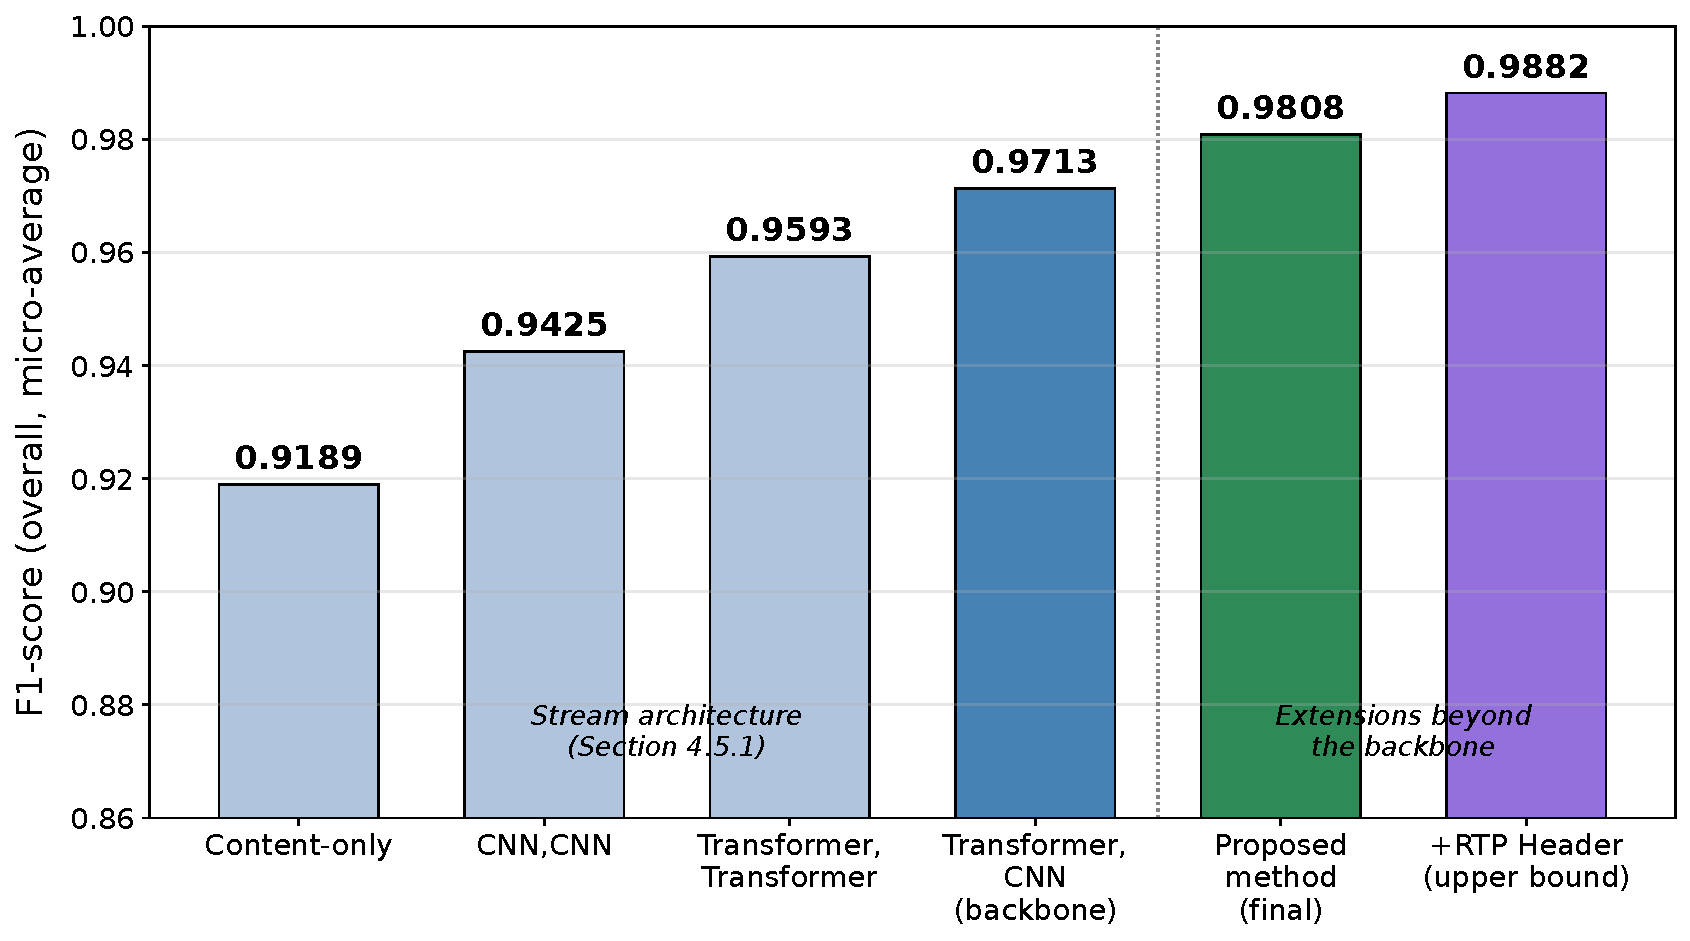
\includegraphics[width=\columnwidth]{figs/ablation_bars.pdf}
\caption{Overall micro-avg F1 across the ablation progression, from the weakest architecture (content-only) to the final proposed method and its protocol-dependent upper bound. Each configuration is evaluated at its own selected threshold, so bars are not directly comparable at a matched operating point (Section~\ref{sec:ablation}). Note the y-axis does not start at zero.}
\label{fig:ablation_bars}
\end{figure}

\subsection{Threshold Sensitivity}
\label{sec:threshold}
Table~\ref{tab:threshold} reports overall and RTP-category F1-scores across percentile thresholds for both positional encoding variants, illustrating how the precision--recall tradeoff shifts with threshold and motivating the selection of $P_{99}$ for the final proposed method.

\begin{table}[!htbp]
\centering
\caption{Threshold sensitivity, sinusoidal (baseline) vs.\ time-aware (proposed) positional encoding -- both on the fixed Transformer-CNN backbone -- evaluated at five percentile thresholds. Overall F1: micro-avg (all 27 files); RTP F1: macro-avg (5 RTP files).}
\label{tab:threshold}
\small
\adjustbox{max width=\columnwidth}{%
\begin{tabular}{lcccc}
\toprule
\multirow{2}{*}{\textbf{Threshold}} & \multicolumn{2}{c}{\textbf{Sinusoidal (baseline)}} & \multicolumn{2}{c}{\textbf{Time-aware (proposed)}} \\
\cmidrule(lr){2-3}\cmidrule(l){4-5}
 & Overall & RTP & Overall & RTP \\
\midrule
$P_{95}$   & 0.9641 & \textbf{0.8226} & 0.9521 & 0.7236 \\
$P_{97}$   & \textbf{0.9713} & 0.7983 & 0.9686 & 0.8052 \\
$P_{99}$   & 0.9277 & 0.1040 & \textbf{0.9808} & \textbf{0.8709} \\
$P_{99.5}$ & 0.9265 & 0.0738 & 0.9668 & 0.7224 \\
$P_{99.9}$ & 0.9225 & 0.0272 & 0.9219 & 0.0327 \\
\bottomrule
\end{tabular}}
\end{table}
Figure~\ref{fig:threshold} visualizes the data in Table~\ref{tab:threshold}. Both variants eventually collapse on RTP detection at sufficiently extreme thresholds ($P_{99.9}$), confirming that no fixed-threshold scheme is collapse-proof; the practically relevant difference is \emph{where this collapse begins relative to each model's own selected operating point}. The sinusoidal-PE model's RTP curve (red, dashed) collapses immediately beyond its selected threshold ($P_{97}$ $\rightarrow$ $P_{99}$), leaving no safety margin, whereas the time-aware model's RTP curve (green, dashed) rises to its maximum at its own selected threshold $P_{99}$ (0.8709), exceeding the best RTP F1 the sinusoidal variant reaches at any swept threshold (0.8226), and only begins declining one step past that point, at $P_{99.5}$. The selected operating point for each variant is marked with a star.

\begin{figure}[pos=htbp]
\centering
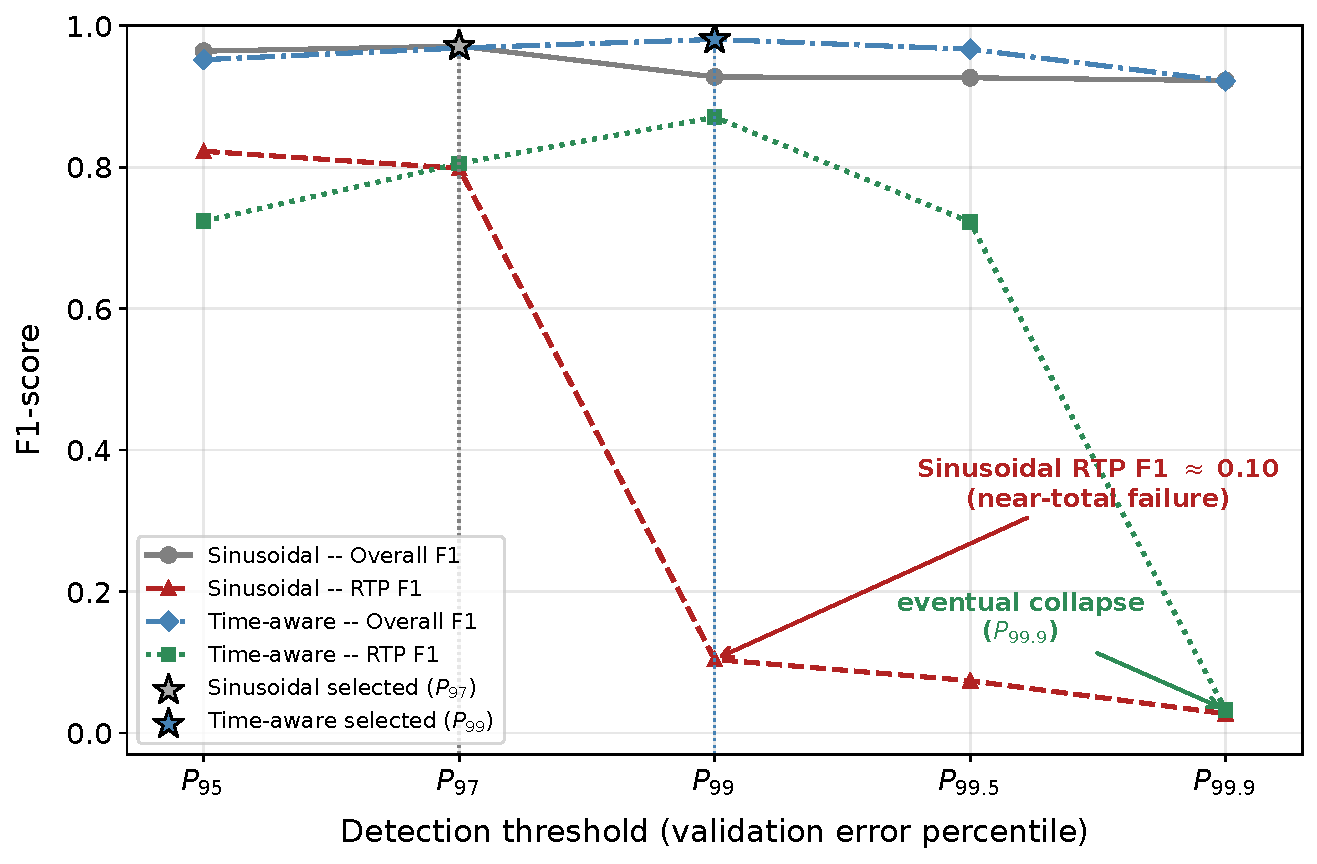
\includegraphics[width=\columnwidth]{figs/threshold_sensitivity.pdf}
\caption{F1-score as a function of detection threshold for the sinusoidal (baseline) and time-aware (proposed) positional encoding variants, shown for both the overall micro-average and the RTP stream replacement category. Stars mark each variant's selected operating threshold.}
\label{fig:threshold}
\end{figure}

The sinusoidal-PE model's overall F1 peaks at $P_{97}$ (0.9713) and then declines by $P_{99}$ (0.9277). This overall decline substantially understates the severity of the underlying failure: broken down by category, RTP stream replacement detection collapses almost completely, from an F1 of 0.7983 at $P_{97}$ to 0.1040 at $P_{99}$ and further to 0.0738 at $P_{99.5}$ and 0.0272 at $P_{99.9}$ -- a regime in which the model fails to detect the overwhelming majority of RTP attacks (average recall drops to approximately 6\% at $P_{99}$ and to roughly 1\% by $P_{99.9}$) while Nmap-based detection remains comparatively unaffected (average recall remains at approximately 98\% at $P_{99}$). This indicates that the sinusoidal model's usable operating range is narrow and asymmetric across attack categories: a threshold chosen based on overall F1 is liable to catastrophically fail on RTP-type attacks just one step higher in the swept grid, with no recovery at any of the higher percentiles evaluated.

The time-aware model exhibits qualitatively different behavior over the range relevant to deployment. Overall F1 continues to \emph{improve} through $P_{99}$ (0.9808, the global peak across all tested percentiles for either variant), with RTP F1 reaching 0.8709 -- exceeding the sinusoidal model's own peak RTP performance across all evaluated thresholds (0.8226, attained at $P_{95}$, one grid step before its selected operating threshold). Performance only begins to degrade one step past $P_{99}$, with a moderate decline at $P_{99.5}$ (RTP F1 = 0.7224) followed by a sharp collapse at $P_{99.9}$ (RTP F1 = 0.0327), reflecting a similarly complete functional collapse to the sinusoidal model's terminal value (0.0272) at the same percentile. This comparison clarifies the nature of the improvement: time-aware encoding does not render the model immune to threshold misspecification -- both variants ultimately fail at sufficiently extreme thresholds -- but it shifts the onset of severe collapse from the very next threshold step (sinusoidal: $P_{97}$ $\rightarrow$ $P_{99}$) to two steps beyond the selected threshold (time-aware: $P_{99}$ $\rightarrow$ $P_{99.9}$, with only a moderate decline at the intermediate $P_{99.5}$), providing a materially larger safety margin against threshold miscalibration in deployment. We select $P_{99}$ as the operating threshold for the final proposed method, as it coincides with the empirical peak of the overall F1-threshold curve in Table~\ref{tab:threshold} and is comfortably within the stable region rather than adjacent to the subsequent collapse observed at $P_{99.9}$.

Beyond motivating this choice, Table~\ref{tab:threshold} also lets us quantify the cost of label-free calibration (Section~\ref{sec:scoring}), in which $p$ is chosen to target a false-positive rate on unlabeled normal traffic alone rather than to maximize F1 on labeled attacks. Under label-free calibration, $p=95$ corresponds to a 5\% FPR. Relative to the labeled-calibration optimum at $P_{99}$ (Overall F1 = 0.9808, RTP F1 = 0.8709), label-free calibration at $P_{95}$ incurs a modest reduction in overall F1 (0.9808 $\rightarrow$ 0.9521, $-2.87$ points) but a substantially larger reduction in RTP-category F1 (0.8709 $\rightarrow$ 0.7236, $-14.73$ points, a relative decrease of approximately 16.9\%), consistent with the asymmetric sensitivity of the RTP category discussed above. Practitioners without access to labeled attacks should therefore expect reliable overall detection at $P_{95}$, with a meaningfully weaker margin specifically for stealthier attack categories such as RTP stream replacement.